
\subsection{Absorbing Markov Chain}
\label{ap:markov}
The subsection explains a well-known fact about absorbing Markov chains, that they converge to an absorbing state with probability one. 
Assume that $\X^m$ form a Markov chain.
In order to reason about this chain we need to consider the transition probabilities. In general, these correspond to our functional approximation scheme. 
Due to the stochastic nature of the Markov chain, we expect to have the variance go up and down. But as the variance decreases, the newly sampled data, due to its finiteness, will be more concentrated, leading in the limit to a set of \ie~a delta functions. This argument assumes that the approximation scheme is good and can converge to delta functions. If not, the errors in approximation may prevent the propagation of errors in stochasticity.



As discussed in the previous section, we can model the process of repeated `sampling' and `fitting' as a Markov chain. In this subsection, we explain how such a process can converge to a stationary state \ie~the absorbing state of a Markov Chain. 
In this derivation we follow Allan Yashinski~\footnote{\url{www.math.umd.edu/~immortal/MATH401/book/ch_absorbing_markov_chains.pdf}}. Suppose we have an absorbing Markov Chain with $r$ transient states $t_1, \dots, t_r$ and $s$ absorbing states $a_1, \dots, a_s$. The whole Markov chain has $r+s$ states, ordered as follows: $t_1, \dots, t_r, a_1, \dots, a_s$. The transition matrix is then defined as 

\begin{equation}
    T = \begin{bmatrix}
            Q & 0_{r\times s}\\
            R & I_s \\
    \end{bmatrix},
\end{equation} 

where
\begin{itemize}
    \item $Q$ is an $r\times r$ matrix holds the probabilities of moving from a transient state to another transient state
    \item $R$ is an $s\times r$ matrix which holds the probabilities of moving from a transient state to an absorbing state. 
    \item $0_{r\times s}$ is the $r\times s$ matrix of all 0's. There 0's represent the probabilities of moving from an absorbing state to a transient state (which is impossible by definition).
    \item $I_s$ holds the probabilities of transitioning between the absorbing states. As transition is impossible, this is just the $s\times s$ identity matrix.
\end{itemize}

We are interested in $\lim_{k\rightarrow\infty} T^{k}(\X_0)$. For a given $k$, the matrix becomes 

\begin{equation}
    T^k = \begin{bmatrix}
            Q^k & 0_{r\times s}\\
            R + RQ + \dots + RQ^{k-1} & I_s \\
    \end{bmatrix} = \begin{bmatrix}
            Q^k & 0_{r\times s}\\
            R\sum^{k-1}_{i=0} Q^{i} & I_s \\
    \end{bmatrix}.
\end{equation} 

Finally, for an absorbing Markov chain with $T = \begin{bmatrix}
            Q & 0_{r\times s}\\
            R & I_s \\
    \end{bmatrix}$, 
    
    we have $\lim_{k\rightarrow\infty} T^{k} = \begin{bmatrix}
            0_{r\times r} & 0_{r\times s}\\
            R(I_r - Q)^{-1} & I_s \\
    \end{bmatrix}$.\\

Since in the limit the transition probabilities to transient states are zero, we end up converging to absorbing states and staying there. In the case of discrete distributions, where we can perfectly approximate a zero-variance dataset (\ie~a delta function), the absorbing states are delta functions centered at any non-zero probability point from the original distribution. In practice, we would like to know the expected number of steps before being absorbed, which may be large. But without knowing our fitting procedure it is impossible to calculate the matrix $Q$ and therefore the average length of time before collapse.

\begin{figure}
    \centering
    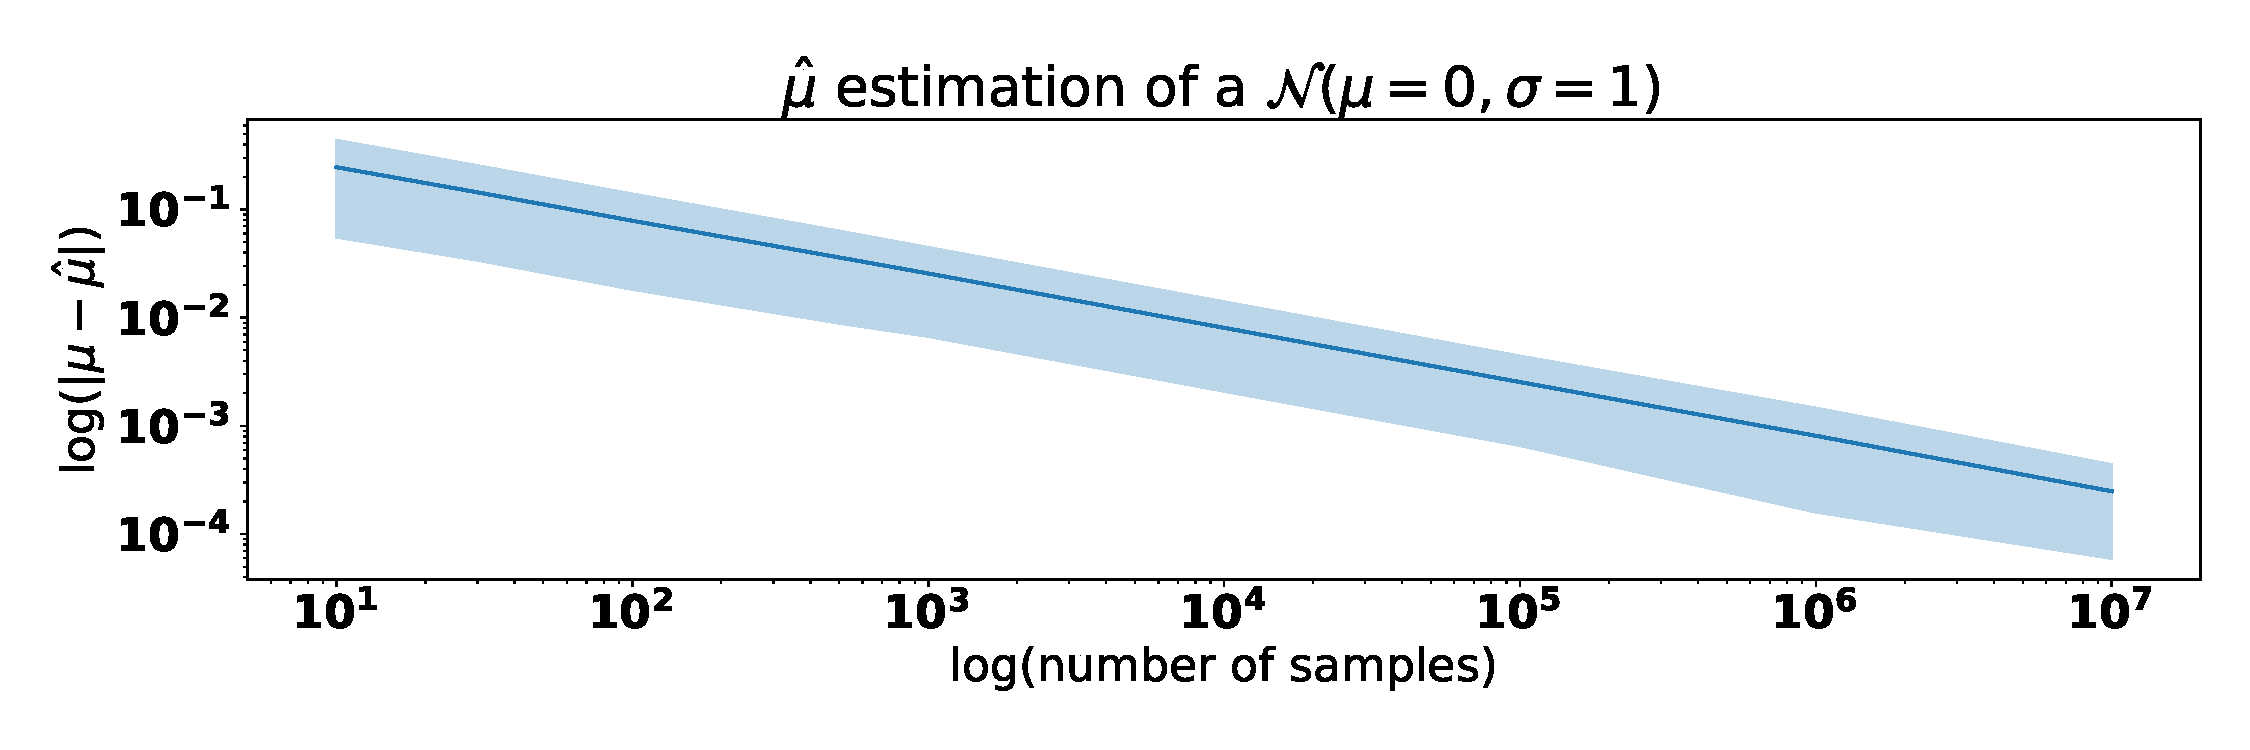
\includegraphics[width=\linewidth]{images/infographics/single_normal_approx.pdf}
    \caption{Approximation of a single-dimensional Gaussian $\mathcal{N}(0,1)$ as a function of number of points. The mean estimator and its standard deviation are calculated from running the procedure 10000 times.}
    \label{fig:single_dim_gaus_approx}
\end{figure}


\begin{figure}
    \centering
    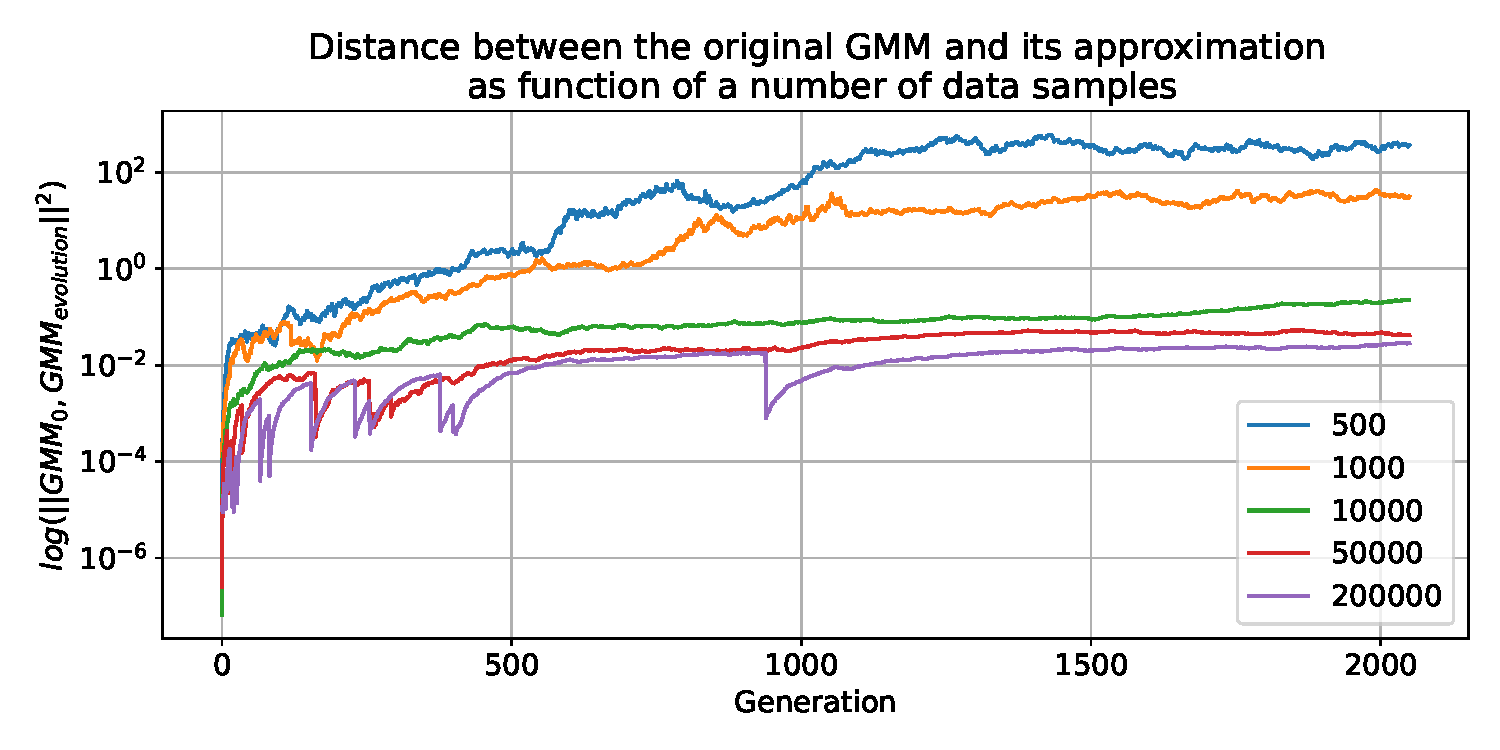
\includegraphics[width=0.9\linewidth]{images/GMM/l2_example.pdf}
    \caption{Progressive fitting of a GMM with different number of samples. On the $y$-axis is shown the logarithm of $L2$ distance between the two GMM distributions. Over the generations the distance begins to grow and can become quite large. The jumps in the distance for large sample sizes occur due to the fixed number of iterations and precision for the expectation maximization algorithm.}
    \label{fig:gmm_l2}
\end{figure}





\subsection{Alternative assumption for noisy approximations}
\label{ap:alternative}
This subsection will cover an alternative assumption, which may be more realistic in \textbf{some} settings, in contrast to assumption 3 from \Cref{sec:noisyapprox}, and this subsection mostly acts as an extension, rather than an alternative. In particular, instead of imposing orthogonality, we can instead impose a certain size requirement on the noise term. This in turn allows us to arrive to a similar result.

To be more precise, we will consider the same setting as in \Cref{sec:noisyapprox}, but we will now replace Assumption 3 with Assumption 3*:

\textbf{Assumptions}:
\begin{enumerate}
    \item[\textbf{3*.}] The extra noise is going to be assumed to be bounded and of the order larger than the sample mean deviation. To be precise we will have a constant $K$ (not dependent on generation $i$), such that for all $i$:
\begin{equation}
    \|\varepsilon_{i+1}\| \leq \frac{K}{M_i}
\end{equation}
\end{enumerate}
Now with the alternative assumption in place, we can follow the exact same calculations to arrive at
\begin{equation}
\label{eq:mean_risk_2_app}
\mathbb{E}\left[R^{i+1}_{W_2}\right]\geq\mathbb{E}\left(\|\mu_{i}-\mu\|^2\right)+\frac{\operatorname{Tr}\Sigma}{M_i}+\mathbb{E}\left(\|\varepsilon_{i+1}\|^2\right)+\frac{2}{\sqrt{M_i}}\mathbb{E}\left((\varepsilon_{i+1})^{\top}\Sigma^{1/2}_iT^{i+1} \right)
\end{equation}
Similar to before, we need to evaluate (which we instead bound this time):
\begin{align}
    \frac{2}{\sqrt{M_i}}\mathbb{E}\left((\varepsilon_{i+1})^{\top}\Sigma^{1/2}_iT^{i+1}\right) 
    &= \frac{2}{\sqrt{M_i}}\int d\Sigma_i\;p(\Sigma_i)\operatorname{Tr}\left[\Sigma^{1/2}_i\operatorname{Cov}(\varepsilon_{i+1},T^{i+1}|\Sigma_i)\right]\neq0\\
    &\geq -\frac{2\sqrt{N}}{\sqrt{M_i}}\int d\Sigma_i\;p(\Sigma_i)\sqrt{\operatorname{Tr}\left[\Sigma_i\Sigma_{\epsilon_{i+1}}\right]}\\
    &\geq -\frac{2\sqrt{N}}{\sqrt{M_i}}\sqrt{\mathbb{E}\left(\varepsilon_{i+1}^{\top}\Sigma_i\varepsilon_{i+1}\right)},\\
    &\geq -\frac{2\sqrt{N}}{\sqrt{M_i}}\sqrt{\frac{K^2\operatorname{Tr}\Sigma}{M_i^2}} = \frac{-2K\sqrt{N}}{M_i\sqrt{M_i}}\sqrt{\operatorname{Tr}\Sigma},
\end{align}
where we used the Cauchy-Schwarz and Jensen inequalities. Note that this is far from optimal inequality, since instead of using the expected value of the largest eigenvalue, we instead bounded it by $\operatorname{Tr}\Sigma$. 
In particular, the per step bound is then:
\begin{equation}
\label{eq:mean_risk_4_app}
\mathbb{E}\left[R^{i+1}_{W_2}\right]\geq\mathbb{E}\left(\|\mu_{i}-\mu\|^2\right)+\frac{\operatorname{Tr}\Sigma}{M_i}+\mathbb{E}\left(\|\varepsilon_{i+1}\|^2\right) - \frac{2K\sqrt{N}}{M_i\sqrt{M_i}}\sqrt{\operatorname{Tr}\Sigma}.
\end{equation}
Without knowledge of the specific values of $K$, $N$ or $\operatorname{Tr}\Sigma$, the best we can do is consider what this means for the bound as $M_i$ becomes large. In particular, contribution from the last two terms will be of order at most $3/2$. As a result we recover a bound similar to all of the ones observed so far:
\begin{align}
\label{eq:mean_risk_3_app}
\mathbb{E}_{\mu_{n+1},\sigma_{n+1}^2}\left[R_{W_2}\right]\geq\operatorname{Tr}\Sigma\left(\frac{1}{M_0}+\frac{1}{M_1}+ \dots + \frac{1}{M_{n}}\right)+\mathcal{O}(3/2)
\end{align}
In particular, we find in the same way, that superlinear scaling would be required to minimise the lower bound on \md~even in the case of more generic models of approximation, in which the mean at step $i+1$ can be separated into the sample mean and an extra bounded term of order at most $1/M_i$. 

\begin{figure}%
    \centering
    \subfloat[\centering Overlaid histograms]{{
\includegraphics[width=0.49\textwidth]{images/lang/norepeat/hist.pdf} }}%
    \subfloat[\centering 3D view]{{
\includegraphics[width=0.49\textwidth]{images/lang/norepeat/3dhist.pdf} }}%
    \caption{Histogram of perplexities of each individual data training sequence produced by different generations as is evaluated by the very first model trained with the real data. Over the generations models tend to produce samples that the original model (trained with real data) is more likely to produce. At the same time, a much longer tail appears for later generations -- later generations start producing samples that would never be produced by the original model~\ie~they start misperceiving reality based on errors introduced by their ancestors. Models here are explicitly forced to not repeat sequences with a penalty of $2.0$. }%
    \label{fig:nonrepeat_hist}%
\end{figure}



\begin{figure}%
    \centering

    \subfloat[\centering \Cref{fig:perp_hist_opt125}.a in 3D. No data preserved.]{{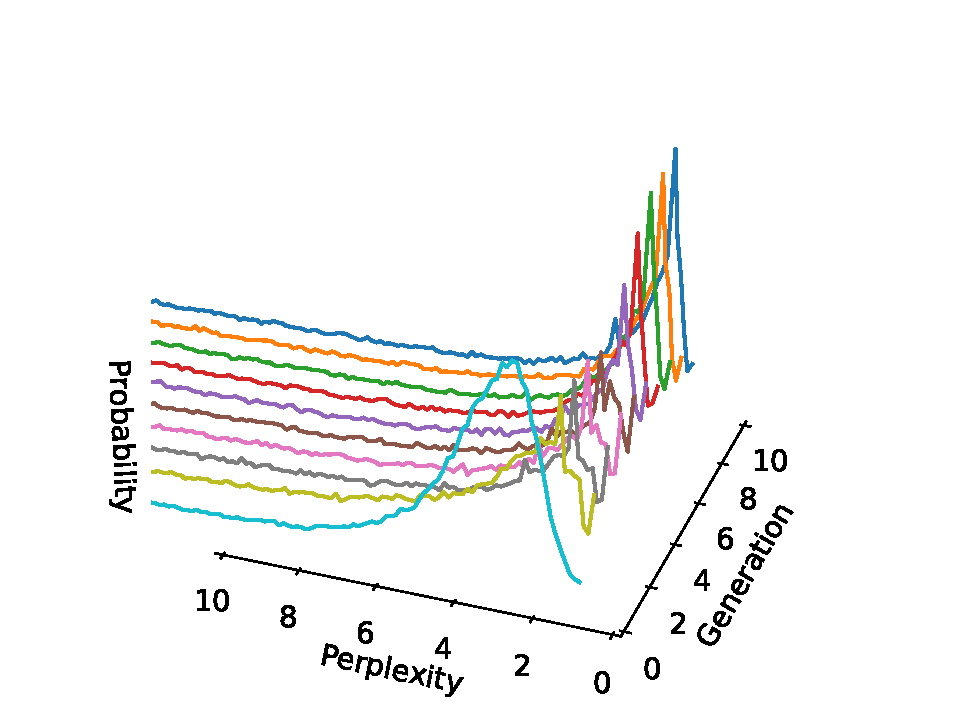
\includegraphics[width=0.49\textwidth]{images/lang/0saved/3dhist.pdf} }}%
    \subfloat[\centering \Cref{fig:perp_hist_opt125}.b in 3D. 10\% original data preserved. ]{{
\includegraphics[width=0.49\textwidth]{images/lang/10saved/3dhist.pdf} }}%
    
    \caption{Histogram of perplexities of each individual data training sequence produced by different generations as is evaluated by the very first model trained with the real data. Over the generations models tend to produce samples that the original model (trained with real data) is more likely to produce. At the same time, a much longer tail appears for later generations -- later generations start producing samples that would never be produced by the original model~\ie~they start misperceiving reality based on errors introduced by their ancestors. }%
    \label{fig:pres_hist}%
\end{figure}
